% LAB 11: Web Scraping
%
% CSE/IT 107: Introduction to Programming
% New Mexico Tech
%
% Prepared by Russell White and Christopher Koch and Tyler Cecil
% Fall 2014
\documentclass[11pt]{cselabheader}
\usepackage{multicol,graphicx}

%%%%%%%%%%%%%%%%%% SET TITLES %%%%%%%%%%%%%%%%%%%%%%%%%
\fancyhead[R]{Lab 11: Web Scraping}
\title{Lab 11: Web Scraping}

\begin{document}

\maketitle

\hrule
\begin{quotation}
``The limits of my language mean the limits of my world.''
\end{quotation}
\begin{flushright}
--- Ludwig Wittgenstein
\end{flushright}

\begin{quotation}
``Any sufficiently advanced technology is indistinguishable from magic.''
\end{quotation}
\begin{flushright}
--- Arthur Clarke
\end{flushright}

\begin{quotation}
``Imagination is more important than knowledge.''
\end{quotation}
\begin{flushright}
--- Albert Einstein
\end{flushright}

\hrule

\section{Introduction}

In this lab, you will be extracting information from web pages and learning how
to plot some of it.

\section{HTML}

As you may be familiar, HTML is the main formatting language of the
Internet.

\section{BeautifulSoup}

What do?

How do?

We gave it to you.

Example

\pagebreak
\section{Matplotlib}

Matplotlib is a neat library for plotting in Python. It works similarly to
MATLAB plotting so that people with experience in that can easily switch over;
however, we will give you our own introduction to it. 

Let's plot the following $x$ and $y$ coordinates:

\begin{table}[!ht]
  \centering
  \begin{tabular}{ llllllllllll }
    \bfseries x & 0 & 2 & 4 & 6 & 8 & 10 & 12 & 14 & 16 & 18\\
    \midrule
    \bfseries y & 0 & 4 & 8 & 12 & 16 & 20 & 24 & 28 & 32 & 36
  \end{tabular}
  \caption{Values for Figure~\ref{fig:x-2x}}
  \label{tab:x-2x}
\end{table}

\begin{lstlisting}[caption={Code to produce Figure~\ref{fig:x-2x}} with values from Table~\ref{tab:x-2x},label={lst:x-2x}]
import matplotlib.pylab as pl

x = range(0, 20, 2)
y = range(0, 40, 4)
pl.plot(x, y, '.')
pl.xlabel('X values')
pl.ylabel('Y values')
pl.title('Random plot of X vs Y')
pl.show()
\end{lstlisting}

\begin{figure}[!ht]
  \centering
  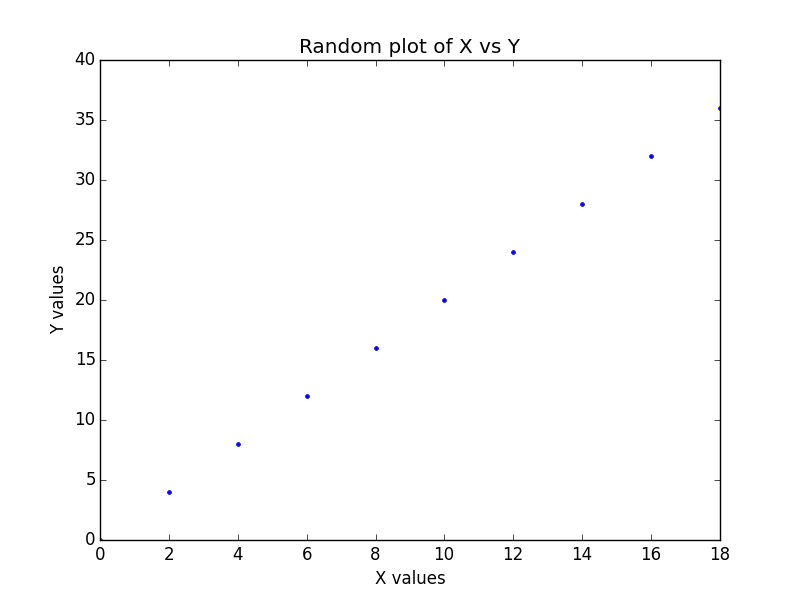
\includegraphics[width=0.8\textwidth]{lab11/x-2x-plot.png}
  \caption{Graph produced by Listing~\ref{lst:x-2x}}
  \label{fig:x-2x}
\end{figure}

The \lstinline!pl.plot()! function takes as arguments a sequence for x, a
sequence for y, and optionally a formatting specifier. The important ones are
``-'' for a solid line and ``.'' for point markers. You can add more options,
such as colors or labels. You can find more docs on
these specifiers on the Matploblib website:
\begin{center}
  \url{http://matplotlib.org/api/pyplot_api.html#matplotlib.pyplot.plot}
\end{center}

You have to call \lstinline!pl.show()! for the graph to actually show. There are
ways to print the graphs to image files, but we are not covering those for now.
You can look them up in the documentation if you want.

Bar plots work in a similar way. The \lstinline!pl.bar()! takes a sequence of
numbers to label the left side of the bars with and a sequence of heights of the
bars.

\begin{lstlisting}[caption={Code to produce Figure~\ref{fig:x-2x-bar}},label={lst:x-2x-bar}]
import matplotlib.pylab as pl

x = range(1, 11, 2)
y = range(1, 21, 4)
pl.bar(x, y)
pl.show()
\end{lstlisting}

\begin{figure}[!ht]
  \centering
  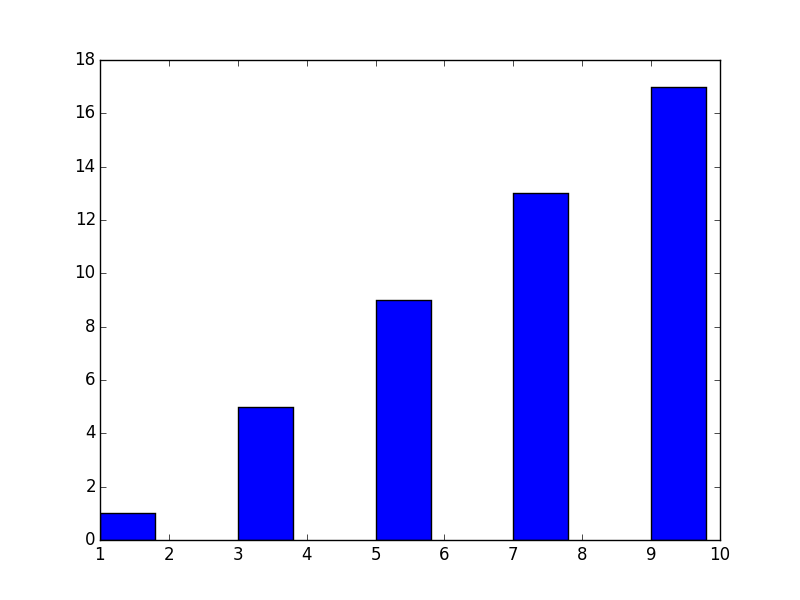
\includegraphics[width=0.8\textwidth]{lab11/x-2x-bar-plot.png}
  \caption{Graph produced by Listing~\ref{lst:x-2x-bar}}
  \label{fig:x-2x-bar}
\end{figure}

These are the two main functions you will need for plotting in this lab. If you
want to customize more, please see the matplotlib pylab documentation at 
\begin{center}
  \url{http://matplotlib.org/api/pyplot_summary.html}
\end{center}

\pagebreak
\section{Wikipedia}

That one thing that russell found (about the philosophy link)

\pagebreak
\section{Exercises}
\label{sec:ex}

%One exerscis for soup (like get the title of a page)
%One for matplotlib (plot x^2)
%The main project

\begin{warningbox}{Boilerplate}
  Remember that this lab \emph{must} use the
  boilerplate syntax introduced in Lab~5.
\end{warningbox}

\begin{description}
  \item[file.py]
\end{description}

\pagebreak
\section{Submitting}

Files to submit:
\begin{itemize}
\item file.py (Section~\ref{sec:ex})
\end{itemize}

You may submit your code as either a tarball (instructions below) or as a .zip
file. Either one should contain all files used in the exercises for this lab.
The submitted file should be named either
\texttt{cse107\_firstname\_lastname\_lab11.zip} or
\texttt{cse107\_firstname\_lastname\_lab11.tar.gz} depending on which method you
used.

For Windows, use a tool you like to create a \texttt{.zip} file. The TCC
computers should have \texttt{7z} installed. For Linux, look at lab 1 for
instructions on how to create a tarball or use the ``Archive Manager'' graphical
tool.

\begin{center}
  \textbf{Upload your tarball or .zip file to Canvas.}
\end{center}

\end{document}
